\section{Results}\label{sec:results}
%Results
%Show effect of colorspaces, blur, annealed mean
%Compare results of architecture (images, error plot, feature maps)
	
In section \ref{sec:method} all the different techniques and methods used resulted in multiple experiments. This sections shows the different results of each experiment, setting the foundation for the discussion.

\subsection{Colorspace}
\begin{wrapfigure}{R}{0.5\textwidth}
	\vspace{-25px}
	\centering
	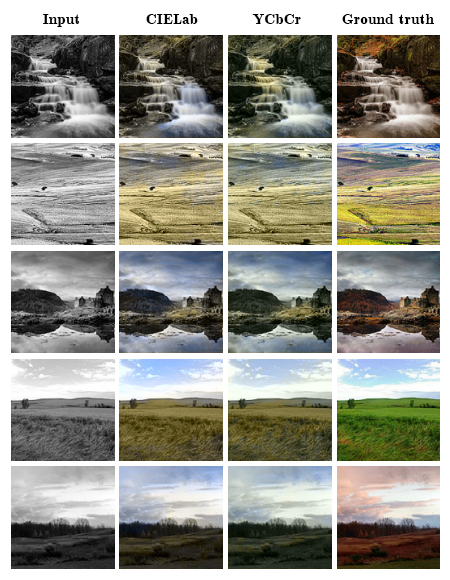
\includegraphics[width=0.42\textwidth]{YCbCr_vs_CIELab}
	\caption{Comparing colorspaces, YCbCr versus CIELab. The output of the compact network architecture trained for 25 epoch on the landscape dataset.}
	\vspace{-37px}
	\label{fig:YCbCr_vs_CIELab}
\end{wrapfigure}
To asses the effect of different colorspaces, a comparison is made between CIELab and YCbCr. The compact network architecture is trained on the landscape set for both the YCbCr and CIELab color space, for a total of 25 epochs. The result is shown in figure \ref{fig:YCbCr_vs_CIELab}. The CIELab colorspace has more saturated colors than the YCbCr output. Similar results were found by Iizuka et al. \cite{IizukaSIGGRAPH2016}.

%\begin{figure}
%	\begin{minipage}{.48\textwidth}
%		
%		\centering
%		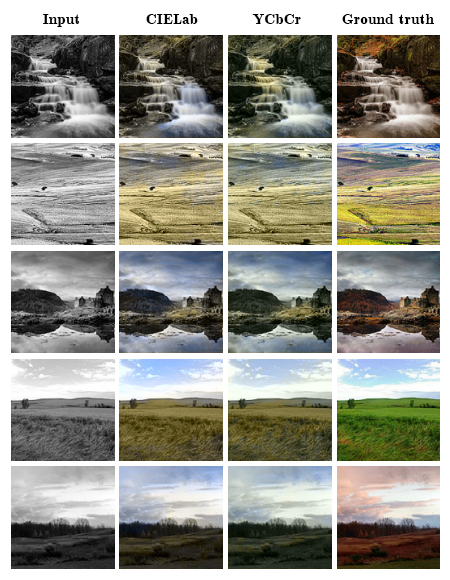
\includegraphics[width=0.78\textwidth]{YCbCr_vs_CIELab}
%		\caption{Comparing colorspaces, YCbCr versus CIELab. The output of the compact network architecture trained for 25 epoch on the landscape dataset.}
%		\label{fig:YCbCr_vs_CIELab}
%		
%	\end{minipage}
%	\begin{minipage}{0.48\textwidth}
%			\centering
%			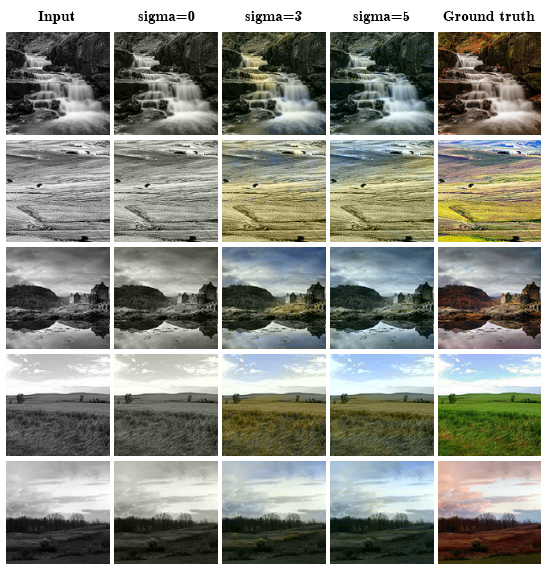
\includegraphics[width=0.95\textwidth]{blur}
%			\caption{The effect of different Gaussian blur kernel sizes to the training of the landscape dataset. The results are from 25 epoch of training.}
%			\label{fig:blur}
%	\end{minipage}
%\end{figure}

\subsection{Gaussian blur}
The comparison between different Gaussian blur kernel size is seen in figure \ref{fig:blur}. The comparison was done with the compact network, trained on the landscape dataset. Note that the Gaussian kernel size is only used during training. Using no blur results in almost zero color output of the network. For $\sigma = 3$ and $\sigma = 5$ the network did learn to colorize images. With $\sigma = 5$ the images look like they have a blue overlay.

\begin{figure}[h]
	\centering
	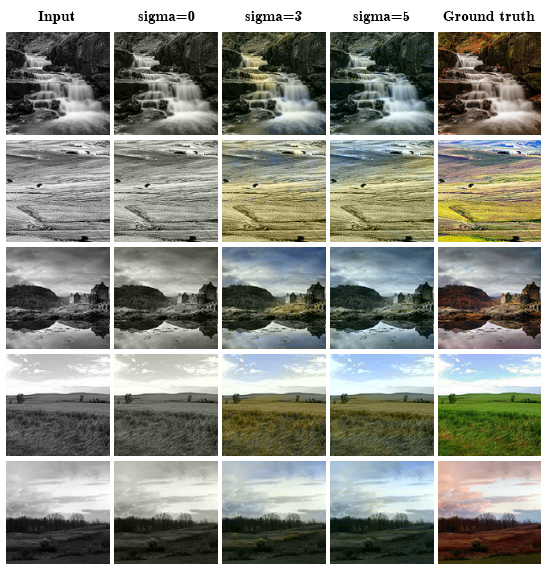
\includegraphics[width=0.6\textwidth]{blur}
	\caption{The effect of different Gaussian blur kernel sizes to the training of the landscape dataset. The results are from 25 epoch of training.}
	\label{fig:blur}
\end{figure}

\subsection{Network output}
In this section the final results of the different CNN architectures is shown. Output images are generated by propagating randomly selected grayscale images of the validation set through the CNNs. The final output images are shown in figure \ref{fig:results}, more results can be found in appendix \ref{ap:more_results}. Note that the annealed mean temperature is set to $0.4$. The optimal setting for the temperature can vary for each network, however the temperature T was held constant for a fair comparison. The compact network output has a lower saturation compared to the other networks. The Compact Classifier Dilated + Concat and VGG16 Classifier show lots of color artifacts. The Compact Classifier and Compact Classifier Dilated show these artifacts to a lesser extend. The images where propagated through the network with trained parameters based on the lowest validation error of all epochs. Some networks showed signs of over fitting. However, the VGG16 Classifier was the most evident, which is shown in figure \ref{fig:overfit}. The error plots of the other architectures can be found in appendix \ref{ap:errors}.
\begin{figure}[h!]
	\centering
	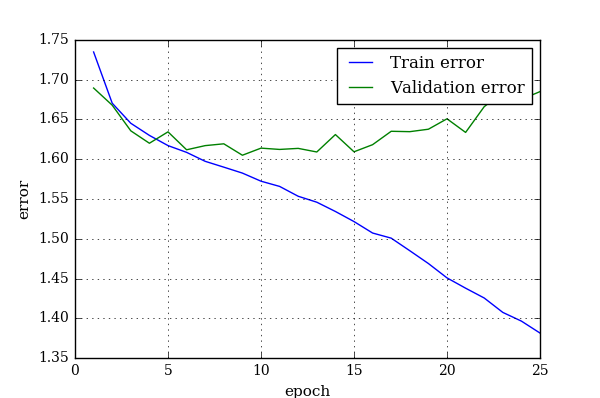
\includegraphics[width=0.5\textwidth]{erros_fruit_Dahl_Zhang_k10_T02_sigma5_nbins20_labda_05_gridsize10}
	\caption{Error plot showing the training and validation error of the VGG16 Classifier network. Note that the error magnitude is different for this network than with the other networks, that is due to the different $\lambda$, even worse results were found while keeping $\lambda$ the same.}
	\label{fig:overfit}
\end{figure}

\clearpage
\begin{figure}[h!]
	\centering
	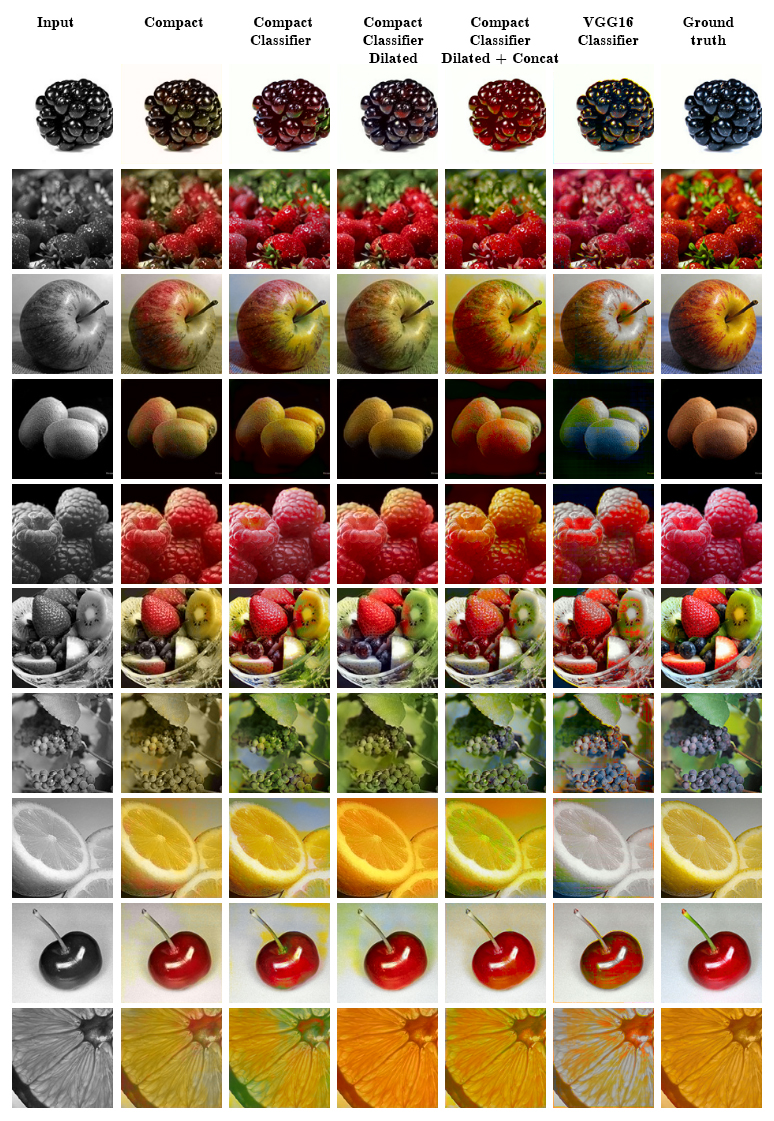
\includegraphics[width=0.9\textwidth]{set2}
	\caption{The results of the different architectures.}
	\label{fig:results}
\end{figure}



